\documentclass{standalone}
\usepackage{tikz}
\usetikzlibrary{arrows,shapes,automata,positioning,intersections,calc}


\begin{document}
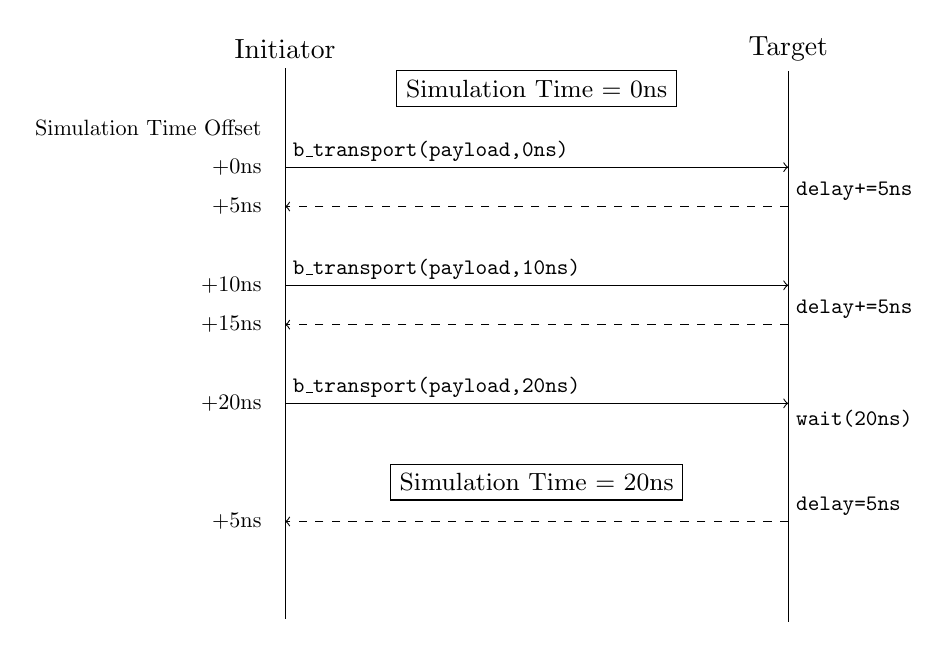
\begin{tikzpicture}

  \node (initiator) {Initiator};
  \node[right=5cm of initiator] (target) {Target};
  \coordinate (a) at ($ (initiator)!.5!(target) $);
  \coordinate (b) at ($ (a) + (0,-5mm) $);
  \coordinate (c) at ($ (a) + (0,-5.5cm) $);
  
  \node[draw] at (b) (time1) {\small Simulation Time = 0ns};
  \node[draw] at (c) (time1) {\small Simulation Time = 20ns};

  \draw (initiator.south) -- ([yshift=-7cm]initiator.south);
  \draw (target.south)    -- ([yshift=-7cm]target.south);

  \coordinate (i1) at ($ (initiator)+(0,-1.5cm) $);
  \coordinate (i2) at ($ (i1)+(0,-5mm) $);  
  \coordinate (i3) at ($ (i2)+(0,-1cm) $);
  \coordinate (i4) at ($ (i3)+(0,-5mm) $);  
  \coordinate (i5) at ($ (i4)+(0,-1cm) $);
  \coordinate (i6) at ($ (i5)+(0,-1.5cm) $);  

  \coordinate (t1) at ($ (target)+(0,-1.5cm) $);
  \coordinate (t2) at ($ (t1)+(0,-5mm) $);  
  \coordinate (t3) at ($ (t2)+(0,-1cm) $);
  \coordinate (t4) at ($ (t3)+(0,-5mm) $);  
  \coordinate (t5) at ($ (t4)+(0,-1cm) $);
  \coordinate (t6) at ($ (t5)+(0,-1.5cm) $);

  \node[anchor=east, scale=0.8] at ([xshift=-2mm,yshift=5mm]i1) {Simulation Time Offset};

  \foreach \i/\j in {1/0,3/10,5/20}{
    \draw[->] (i\i) node[anchor=east,scale=0.8] at +(-2mm,0) {+\j ns} node[anchor=west,scale=0.8] at +(0,2mm) {\texttt{b\_transport(payload,\j ns)}} -- (t\i);
  }
  
  \node[anchor=west,scale=0.8] at ([yshift=-2mm]t5) {\texttt{wait(20ns)}};

  \foreach \i/\j/\k in {2/5/+=,4/15/+=,6/5/=}{
    \draw[->,dashed] (t\i) node[anchor=west,scale=0.8] at +(0,2mm) {\texttt{delay\k 5ns}} -- (i\i) node[anchor=east,scale=0.8] at +(-2mm,0) {+\j ns};
  }


\end{tikzpicture}
\end{document}



